% !TEX root = ../thesis_main.tex
\chapter{Results}\label{chap:results}
    As a large part of this work consisted of hardware design and manufacturing, the results section is split into hardware development results and measurement results obtained \textit{with} that hardware as well as commercially available machines. Additionally, simulation results will be added as a separate section in the end of this chapter.
\section{Hardware}
    This section will cover the results concerning the hardware built in the course of this thesis. This also covers calibration results as well as performance measurements of single components. If results were acquired by the workshop, this will be clearly indicated.
    \subsection{Parahydrogen generator}
        The rebuild of the parahydrogen generator with more fixed lines and less dangling connections works more reliably with one leak in the course of this work compared to one every few months before. The whole setup was moved to another building without any loss in performance or reliability despite complete dis- and reassembly.
        Performance of the helium recondenser was unchanged over the years cooling the system down in \SI{2\pm0.3}{\hour}. Filling a \SI{1.5}{\l} to \SI{50}{\bar} takes \SI{1.5}{\hour} setting the needle valve to flows of \SI{2}{\liter\per\hour}. The smaller \SI{0.5}{\liter} bottle takes only about \SI{0.9}{\hour} to fill.
        Parahydrogen was quantified and showed an enrichment of \SI{95\pm3}{\%} directly after production. The decay constant inside the high pressure aluminium bottles was in the range of days: $\mathrm{T}_{1/2} = \SI{5.4\pm 0.8}{\day}$
    \subsection{Low field NMR}
    The setup used in most low field experiments in this work was the low field spectrometer or low field NMR (see section \ref{sec:matMeth:lowFieldSpectrometer}). After manufacture, partly during this work and partly after, the setup needed to be assembled, calibrated and shimmed and experiments with different substances and in various settings were performed and are described in the following sections.
        \subsubsection{$\mathbf{B_0}$ coils}
        Preexisting solenoid coils were used to generate the static magnetic field, later more were manufactured in the course of this work in an effort to generate more homogeneous fields. The $\mathrm{B_0}$ coils exhibit field distributions (and thus frequency distributions) as well as  linewidths in the order of magnitude predicted by the simulations (section \ref{sec:results:sim}). Through manufacturing errors and changes to the coil during long term use, the linewidths deteriorated over time. It is important to note that, at currents above $\SI{1}{\ampere}$, the $\mathrm{B_0}$ coil heated noticeably. While the heating itself is unproblematic, the resulting expansion of the materials leads to an overall elongation of the coil and thus lower fields. The coil position is especially relevant, ferromagnetic materials close to the coil bore disturb the field homogeneity (e.g. table legs made from steel under the wooden tabletop).
         \subsubsection{Shims and programmable power supply}
         A linear shim system for all three spatial dimensions was successfully built and installed at the low field spectrometer.
         The three linear shims are adjustable via a programmable power supply and show the expected effect which is described here. The rotational position of the receive coil is relevant to the shims indicating they're working as intended (i.e. x- and y-shim currents need to be exchanged while z shim remains unchanged on a \SI{90}{\degree} rotation) . Manual shimming results are shown in figure \ref{fig:results:lowFieldSpectrometer:shims}. The optimal results were achieved for currents of \SI{0}{\milli\ampere},  \SI{0}{\milli\ampere} and \SI{0}{\milli\ampere} for x-, y- and z-shim respectively. Using the added shim tool \ref{sec:matMeth:hypercontrol}, line widths were reduced from $\approx \SI{250}{\hertz}$ to $\approx \SI{30}{\hertz}$ in the case of large samples of $\approx $\SI{40}{\milli\litre}. If the initial field was generated by a less homogeneous, more asymmetric coil in which no signal was visible without shims, signal was discovered after shimming and the optimal linewidth reached was $\approx \SI{50}{\hertz}$.
            \begin{figure}
                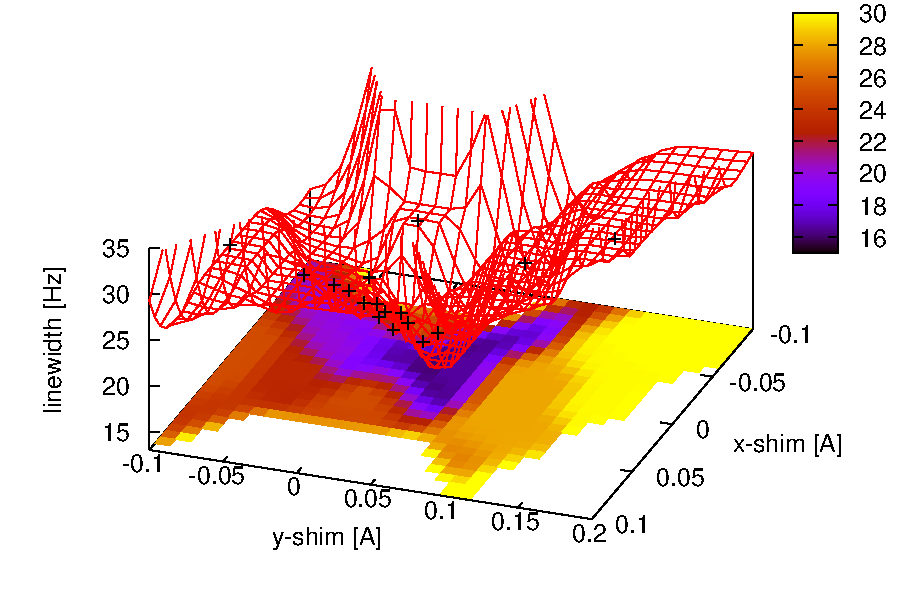
\includegraphics[width=0.99\textwidth]{/figures/experiments/lowFieldSpectrometer/shims/shimXY.pdf}
                \caption[Manual low field shimming]{Linear shimming in x- and y-directions. Shimming was done manually: $^{1}$H spectra of water were recorded and evaluated as to their linewidth. Later, automatic shimming was implemented (see section \ref{sec:matMeth:shims}). Black dots indicate actual measurement points, the red mesh is a spline interpolation of the measurement data. The same interpolation is shown as a colormap on the bottom of the graph where black color corresponds to narrowest lines and thus highest homogeneity.}
                \label{fig:results:lowFieldSpectrometer:shims}
            \end{figure}
            The automatic calculation of the linewidth of a given measurement works well and yields results similar to the ones of a manual adjustment with significantly less user interaction. The method for linewidth determination described in section \ref{sec:matMeth:hypercontrol} based on interpolation yields linewidths within \SI{10}{\percent} of the fitted result if the SNR is sufficient, i.e. if the maximum value in the spectrum can clearly be attributed to the nuclear resonance in question. This may require a frequency selection to exclude noise induced peaks, while the low chemical shift resolution at low fields usually eliminates the need for 
        \subsubsection{Receive coil and $\mathrm{B_1}$ coil}
        \label{sec:results:receiveCoil}
        Receive circuits were designed according to section \ref{sec:matMeth:receiveCoil}. They provided a Q-factor (see section \ref{sec:matMeth:receiveCoil} for definition) of 128 as shown in figure \ref{fig:results:networkAnalysis}.  An additional, higher frequency resonance with Q-factor of 32 can be seen to the right in the same plot at around \SI{460}{\kilo Hz}. The second graph shows the same measurement performed with the untuned saddle coil. The latter shows no significant dips and is thus considered broadband, i.e. as long as the RF-amplifiers power is sufficient, it can be used at arbitrary frequencies. Note that additional impedances are introduced into the system through the connection to the NI DAQ interface that cannot be neglected especially in the higher frequency range above $\SI{100}{\kilo\hertz}$ where the coil's intrinsic capacities are comparatively small. A measurement similar to the network analyzer measurement is shown in figure \ref{fig:results:niNetworkAnalysis}. In this case, an RF-pulse was transmitted from the National Instruments card via the broadband $B_1$ coil and the resulting signal in the receive coil is recorded. Compared to the network analyzer measurement, a frequency shift can be observed, the peak previously visible at slightly above \SI{200}{\kilo\hertz} is now visible at \SI{70}{\kilo\hertz}. The Q-factor calculated from this data is different - 30 and 440 - from the one measured in the external measurement with the network analyzer.
            \begin{figure}
                \centering
                %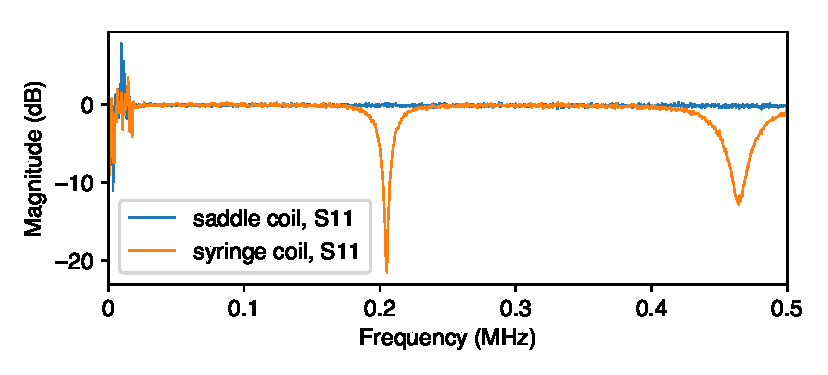
\includegraphics[width = 0.95\textwidth]{/figures/experiments/lowFieldSpectrometer/networkAnalysis.pdf}
                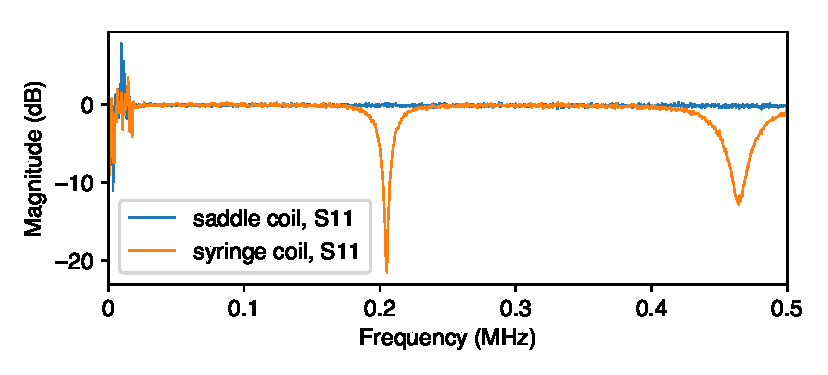
\includegraphics[width = 0.99\textwidth]{/figures/experiments/lowFieldSpectrometer/networkAnalysis.pdf}
                \caption[Network analysis receive coil]{Network analysis frequency of a receive coil (orange) and saddle transmit coil (blue) commonly used in the low field experiments and a corresponding transmit coil. Note the strong dip in the syringe receive coil at around \SI{210}{\kilo\hertz} that was intended to receive the NMR signal as well as the second, lower and broader resonance at around \SI{470}{\kilo\hertz}. In contrast to that, the broadband transmit coil displayed in blue shows a flat frequency response.}
                \label{fig:results:networkAnalysis}
            \end{figure}
            \begin{figure}
                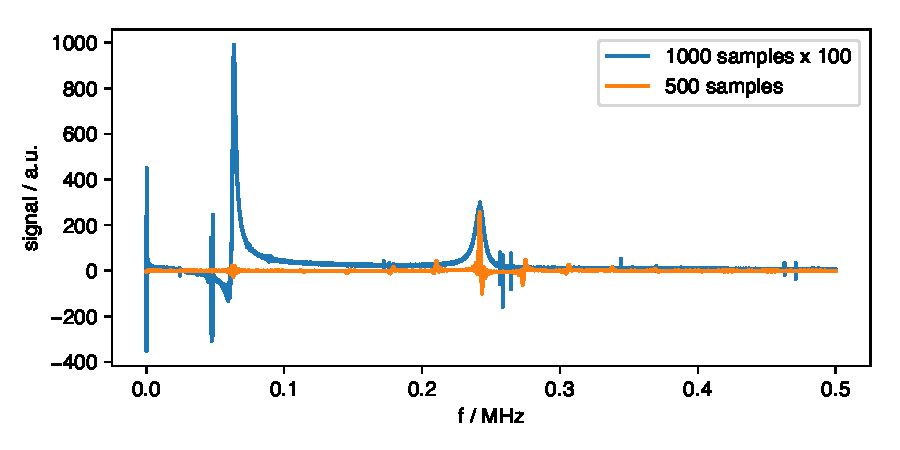
\includegraphics[width = 0.95\textwidth]{/figures/experiments/lowFieldSpectrometer/niNetworkAnalysis.pdf}
                \caption[Network analysis NI card]{ADC result of a pulse transmitted to the tuned receive coil (blue). The central peak shows the resonance frequency of the coil employed for the measurements. In contrast to the network analysis measurement (fig. \ref{fig:results:networkAnalysis}), the lower  order resonance can now be seen to the left at around \SI{70}{\kilo\hertz}. Note the strong frequency shift due to the different downstream receive circuit.}
                \label{fig:results:niNetworkAnalysis}
            \end{figure}
            For the measurement with the National Instruments card, a strong frequency shift of the two peaks is observed. The peak intended for signal reception is shifted to frequencies of around \SI{70}{\kilo\hertz} while the peak to its right is shifted to \SI{240}{\kilo\hertz}. This resonance was then used for subsequent proton measurements at $\approx\SI{5}{\milli\tesla}$. Dual resonant coils for $^{1}$H and $^{13}$C signal reception showed a less prominent dip in both channels, while the secondary channel (1H in most cases, section \ref{sec:matMeth:oscillatoryCircuits}) was affected more strongly by the adapted circuitry.
    \subsection{Sabre shuttling system}
    As the combination of continuously hyperpolarized substances and biological materials proved difficult, a high batch polarization - preferably on X-nuclei was pursued. As SABRE polarization of the chosen $^{15}$N tracers is only possible at nanotesla fields, a system was built to serve both as a polarizer and as a transfer unit. The system designed to transfer a sample between the magnetic fields for polarization and measurement within seconds works as intended. Fluid losses are about \SI{25}{\percent} within \~15 shuttling cycles at high flow rates of \SI{20}{\litre \per\hour} and long bubbling times of 30 seconds per measurement i.e. \SI{8}{\minute} of pH$_2$ flow through the sample. These losses were deemed acceptable for the intended batch production of hyperpolarized tracers. The bubbling system supplies pH$_2$ to the solution in amounts large enough to generate polarization levels in the single digit percent range \ref{fig:results:15N:polarization}.
        \subsubsection{15N coil}
    The coil for $^{15}$N signal reception was matched and tuned to fit the requirements of the \SI{9.4}{\tesla} small animal imager used for detection. The network analyzer showed a Q-factor of $\frac{\SI{405}{\mega\hertz}}{\SI{40}{\mega\hertz}} = \SI{10}{}$ with a width of \SI{40}{\mega\hertz} at half maximum. Inside the small animal NMR, similar resonance widths of nn were observed while the attenuation was \SI{23}{\deci\bel}. Clear signal was visible using the $^{15}$N glycine (sec. \ref{sec:matMeth:15Ncoil}) phantom in a single shot measurement. Shimming reduced linewidths of the phantom to \SI{10}{\hertz}. Linewidths of the hyperpolarized $^{15}$N pyridine signal were in the range of \SI{30}{\hertz} without explicit shimming for the sample's geometry and content which differ significantly from the glycine phantom.
                \begin{figure}
                    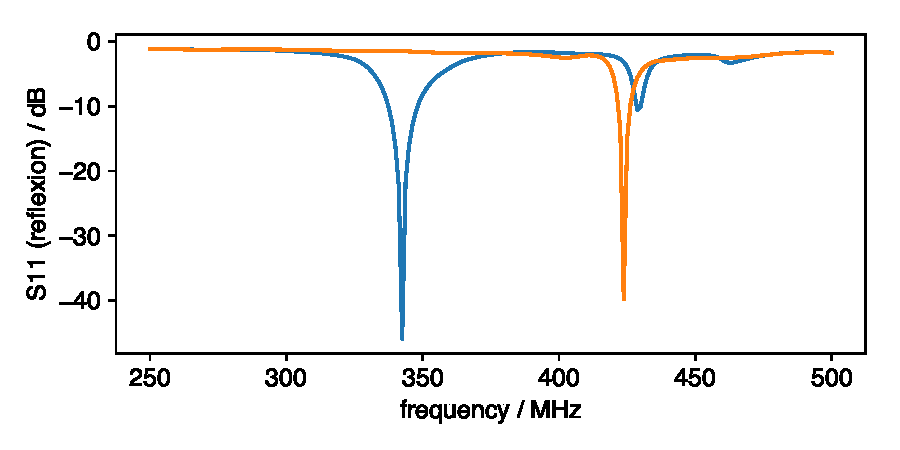
\includegraphics[width=0.99\textwidth]{/figures/experiments/15NSabre/15Ncoil.pdf}
                    \caption[15N coil network analysis]{The range of frequencies covered by high field $^{15}$N detection solenoid coil built for the hyperpolarized experiments. Due to the large range of the tune capacitor, the range was large enough to cover \SI{100}{\mega\hertz} with matching capacities in the \SI{40}{\deci\bel} range.}
                    \label{fig:results:15N:networkAnalysisCoil}
                \end{figure}
        \subsubsection{Flip angle calibrationion}
            The flip angle for the $^{15}N$ coil could not be calibrated automatically which is why it was manually calibrated. To achieve equidistant excitation voltages, the pulse power, that is proportional to the second power of the voltage, needed to be varied in non-linear steps. Additionally, the power is given in dB increasing non-linearity. Equidistant steps were thus calculated via:
            \begin{equation}
                \Delta dB = 10\cdot \log_{10}(\Delta V^2)
            \end{equation}
            Figure \ref{fig:results:15N:flipAngle} shows the results of that calibration, both over dB and over voltage. The signal area of the 15 N -Glycine phantom measured in the 15 N coil is  plotted over relative voltage and attenuation in dB. The voltage data is used to fit a sine and to find the \SI{90}{\degree} flip angle. The \SI{90}{\degree} angle is marked by a vertical line for both the voltage and attenuation plot. 
            \begin{figure}
                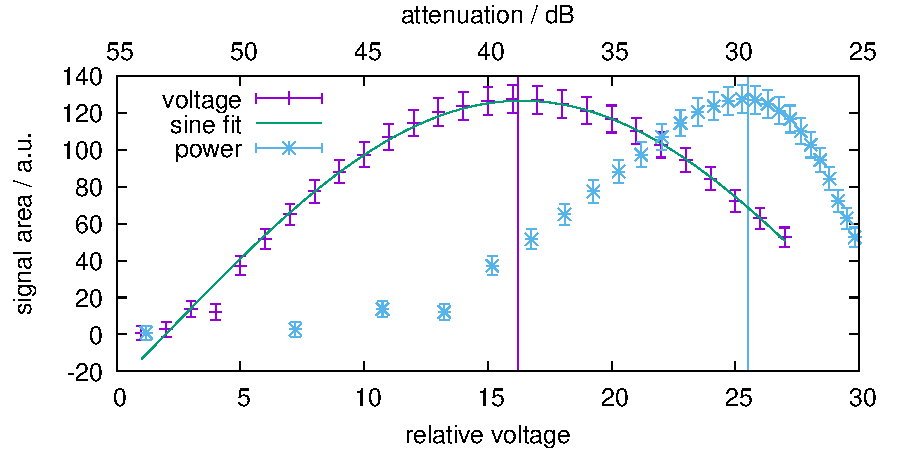
\includegraphics[width=0.99\textwidth]{/figures/experiments/15NSabre/flipAngle/faDiss.pdf}
                \caption[Flip angle calibratin 15N]{Signal area of the $^{15}N$-Glycine phantom measured in the $^{15}N$ coil plotted over relative voltage and attenuation. The plot over relative voltages fit with a sine to find the \SI{90}{\degree} flip angle. The \SI{90}{\degree} angle is marked by a vertical line for both the voltage and attenuation plot.}
                \label{fig:results:15N:flipAngle}
            \end{figure}
        \subsubsection{Parahydrogen supply}
        The newly constructed bubbling disk (see section \ref{sec:matMeth:lowFieldReactor}, specifically figure \ref{figure:materialsMethods:probesPSU}) showed to provide hydrogen to the sample more homogeneously than the previously used single hole supply. Different hole sizes or numbers of holes can provide similar flow for samples of different viscosities. The widening of the cylinder towards the top provides enough space for bubbles to burst and reduces fluid losses due to minimizing sample splashing into the venting line and being lost irrecoverably.
        \subsubsection{Pressure stability}
        To ensure a safe operation, the pressure stability of the devices was estimated via Autodesk Inventor simulations. The low field reactor's results are shown here.
        The simulated pressure deformation of the vessels was \SI{200}{\bar}. A factor of safety of $\gamma = 4$ was deemed appropriate for the setup. As expected, the most vulnerable part is the long side of the cylinder (see figure \ref{fig:results:bubblingReactorPressure}), but wall thickness of \SI{3}{\milli\meter} suffices for a factor of safety of 4 if the setup is operated at a maximum pressure of \SI{50}{\bar}. Experimentally, the pressure resistance of \SI{50}{\bar} was confirmed; no problems concerning material fatigue were observed within a few thousand pressure cycles. Figure \ref{fig:results:bubblingReactorPressure} shows the displacement of the different parts at \SI{200}{\bar}. The maximum displacement is in the range of \SI{0.25}{\milli\meter} and is within the yield strengths of PSU given in table \ref{figure:materialsMethods:probesPSU}. For practical reasons (complicated manufacturing process), the burst pressure was never  validated experimentally.
            \begin{figure}
                \centering
                \subfloat[Overall displacement\label{fig:results:sim:pressure:displacement}]{\includegraphics[width = 0.49\textwidth]{/figures/simulations/15NSabre/displacement200.eps}}
                \hfill
                \subfloat[X displacement\label{fig:results:sim:pressure:xDisplacement}]{\includegraphics[width = 0.49\textwidth]{/figures/simulations/15NSabre/xDisplacement200.eps}}\\
                \subfloat[Y displacement\label{fig:results:sim:pressure:yDisplacement}]{\includegraphics[width = 0.49\textwidth]{/figures/simulations/15NSabre/yDisplacement200.eps}}
                \hfill
                \subfloat[Z displacement\label{fig:results:sim:pressure:zDisplacement}]{\includegraphics[width = 0.49\textwidth]{/figures/simulations/15NSabre/zDisplacement200.eps}}
                \caption[Reactor wall stress simulations]{Wall stress of the low field reactor for a pressure of \SI{200}{\bar}. (a) shows the overall displacement while (b), (c) and (d) show the displacement in X-, Y-, and Z-direction, respectively. The yellow arrows shown in pairs of four indicate the areas where pressure was applied in the simulation.}
                \label{fig:results:bubblingReactorPressure}
            \end{figure}
            Chemical resistance to methanol- and ethanol-pyridine mixtures was as good as expected, though resistance to neat pyridine is not given. While there was never any problem with the pyridine concentrations  up to \SI{30}{\micro\Molar} used in the experiments, a neat pyridine batch showed to dissolve the PSU casing (see \ref{sec:discussion:componentsAndDurability}).
        \subsubsection{Mu metal shielding}
        To reach the nanotesla fields for effective hyperpolarization, the sample needed to be shielded from the earth magnetic field. The three layered mu metal shield purchased for that purpose reduced fields to \SI{50}{\nano\tesla} inside the magnetic stray field of about \SI{50}{\milli\tesla} of the \SI{9.4}{\tesla} small animal MRI. In earth magnetic field, fields inside the shield went down even further to the fluxgate's measurement limit in the single digit nanotesla fields. Manual degaussing (see section \ref{sec:matMeth:degaussing}) was prone to errors and left the shields in different, non-comparable states (i.e. different residual fields were measured inside the shielding directly after degaussing). The workshop-built, automatic degaussing power supply was capable of reducing those errors and a reproducible residual field of \SI{50}{\nano\tesla} was produced. The current's slew rate of \SI{0.25}{\ampere\per\second} showed to be sufficient in combination with an initial current of \SI{7}{\ampere}. The adaption to other shield sizes works automatically after a single calibration run and was tested using a smaller shield requiring lower degaussing currents.
        \subsubsection{Low field manipulation}
        As the magnetic shielding of the MuMetal is static but an adaptation of the field inside was necessary to set optimal polarization parameters, the dual helmholtz assembly described in section \ref{sec:matMeth:Helmholtz} was set up so it fits inside the shields. The field inside the Mu Metal shielding was measured without any current flowing in the B0 coil as well as with the coil turned on. Measurements showed different results for the solenoid coil used at first and the later installed Helmholtz coil. Both coils were used to measure fields at the reactors position shown in figure \ref{figures:results:helmholtzCoilsCenterField}. As the resolution of the current for the power supply used was \SI{0.1}{\milli\ampere} resulting in field steps in the range of \SI{213\pm 31}{\nano\tesla}, an additional \SI{10}{\kilo\ohm} resistor was used to reduce the current by a factor of $\sim 1000$ (the coil's resistance is $\sim \SI{10}{\ohm}$). The power supply could thus not be used in constant current mode but a voltage had to be set introducing a larger error to the current, but allowing for much smaller adjustments to the current. Results that show the highly linear dependence of current (or voltage, ohmic dependency) and magnetic field are plotted in figure \ref{figures:results:helmholtzCoilsCenterField}. The slope of the field-voltage fit is steeper for the solenoid compared to the Helmholtz coil as shown in the inset of figure \ref{figures:results:helmholtzCoilsCenterField}. Both changes and absolute values of $B_{xy}$ are small compared to $B_z$ over the complete range displayed (an exception being the current- and field free central point). This leads to a dependence between voltage and field of
            \begin{equation}
                B(U) = 111.3\pm 0.1 \si{\nano\tesla\per\volt} - 79.1 \si{\nano\tesla}
            \end{equation}
            for the Helmholtz coil and
            \begin{equation}
                B(U) = 333.3 \frac{\si{\nano\tesla}}{\si{\volt}} - 168 \si{\nano\tesla}
            \end{equation}
            for the solenoid coil.
                \begin{figure}
                    \centering
                    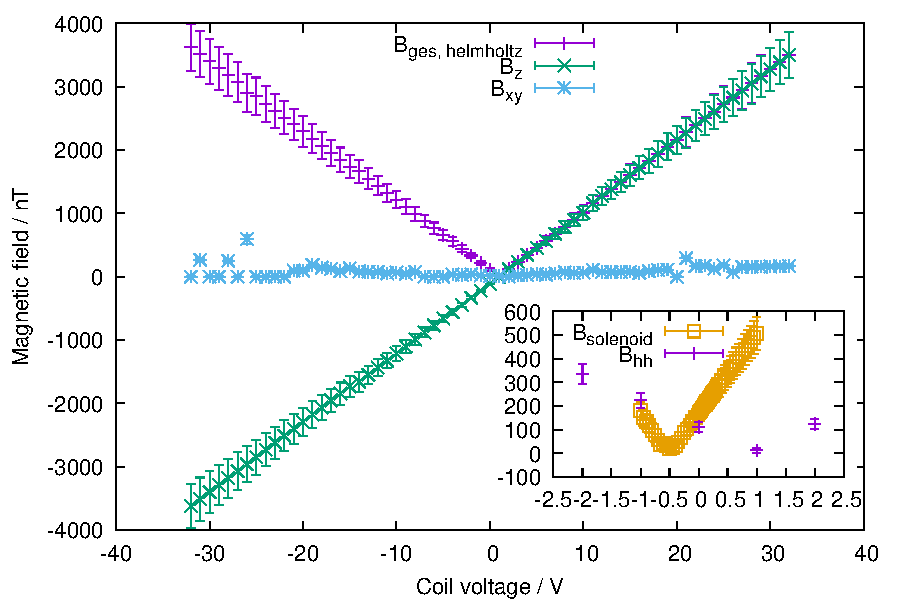
\includegraphics[width=0.99\textwidth]{/figures/experiments/helmholtzCoils/fieldHelmholtzCoils.pdf}
                    \caption[Helmholtz fields]{Calibration of the voltage (and thus current) to reference actual fields using the fluxgate sensor and ramping trough the voltages in both polarities. In the insert, the fields of the previously used solenoid coil can be seen in comparison to the Helmholtz coils' field in the central region. Its slope is steeper than the Helmholtz coils'. Voltage is applied to the inner Helmholtz coil pair via a \SI{10}{\kilo\ohm} resistor to limit currents to values below the power supply's resolution.}
                    \label{figures:results:helmholtzCoilsCenterField}
                \end{figure}
        \subsubsection{Shuttling reproducibility}
            \label{results:15N:shuttlingReproducibility}
            Two things were important concerning the shuttling process itself: No sample should remain on the high field side, so that polarization was correctly estimated and the shuttling process should be reproducible, i.e. the same volume should arrive at the high field side ech shuttling cycle.
            To ensure that the sample can be removed completely from the high field side (sec. \ref{sec:matMeth:highFieldProbe}), spectra in both 'states' of the system (i.e. with the high field probe container filled and emptied) were recorded (figure \ref{fig:results:15N:shuttlingRemoval}). The residue left in the high field chamber after the shuttling procedure does not generate an observable signal. To be able to estimate the empty containers maximum signal, the noise level was measured after maximizing the its integral through phase shifts. The signal ratios lower limit $\frac{I_{in}}{I_{out}}$ can be estimated and corresponds to a maximum fluid volume of \SI{0.01}{ml} remaining in the high field chamber. Considering that this fraction is completely unpolarized, the overall polarization of a \SI{3}{ml} sample that is added to the sample remained at high field  will be reduced by \SI{0.5}{\percent} \ref{fig:results:15N:shuttlingReproducibility}.
            \begin{figure}
                \centering
                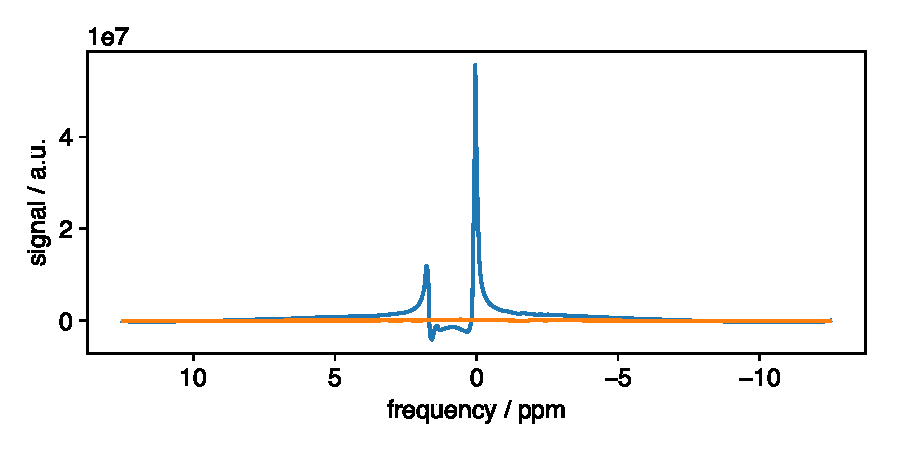
\includegraphics[width=0.99\textwidth]{/figures/experiments/15NSabre/reproducibility/spectraComparisonShuttle.pdf}
                \caption[High field removal efficiency]{1H spectra of the high field reactor in the filled (blue) and empty (orange) state. The filled state delivers a lot more signal as expected while the integration over the empty state spectrum shows a signal reduction of 3000.}
                \label{fig:results:15N:shuttlingRemoval}
            \end{figure}
            To test the reproducibility of the shuttling system, a hyperpolarized $^{1}$H pyridine sample was shuttled back and forth multiple times. The result of this measurement is shown in figure \ref{fig:results:15N:shuttlingReproducibility}. It can be seen that even with high flows of \SI{40}{\litre\per\minute} used for testing the reproducibility and extensive bubbling times of \SI{30}{\second} per measurement, the signal drops to only \SI{75}{\percent} after 15 shuttling procedures. Note that the actual losses may be even smaller as temperature effects which may arise due to methanol evaporation at high flow rates are neglected in this measurement, but have been shown to have an effect on signal intensity in separate experiments. Using the shuttling setup, temperatures in the sample could be reduced from ambient temperatures of \SI{20}{\celsius} to \SI{2}{\celsius} within \SI{5}{\min}. Further increasing the flow even decreased temperatures to below \SI{0}{\celsius}.
            \begin{figure}
                \centering
                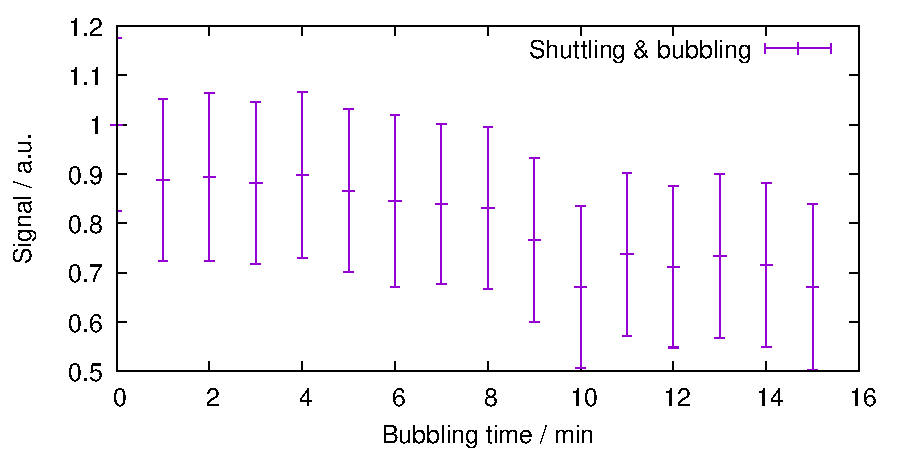
\includegraphics[width=0.99\textwidth]{/figures/experiments/15NSabre/reproducibility/bubblingLosses.pdf}
                \caption[Bubbling fluid losses]{Signal intensity during multiple minutes of hydrogen bubbling using a $^{1}$H hyperpolarized pyridine sample. Note that the signal drops to about \SI{70}{\percent} of its initial value after 8 minutes of continuous hydrogen supply.}
                \label{fig:results:15N:shuttlingReproducibility}
            \end{figure}
    \subsection{Fluxgate readout electronics}
    To measure fields in the nanotesla range, a magnetic fluxgate sensor was purchased and readout electronics were designed and built in this work. The readout electronics were designed to feature a wide range of amplifications for all three spatial dimensions to achieve high resolution measurements at low magnetic fields while maintaining the full measurement range. A 24 V DC power supply was combined  with a bidirectional DC-DC-converter to provide the $\pm\SI{15}{\volt}$ to supply power to the fluxgate. Additionally a PCB board was fitted with the electric parts of the readout electronics (see \ref{sec:matMeth:teensyShield}). For testing purposes, a simple program using serial in and output to toggle the analog switches on the board was written. All switches were successfully tested to work, though three had to be replaced at some point due to malfunction. Probably, this was due to damage during assembly or short circuits during testing as the board is now working as expected for about 1.5 years.
    \subsection{Fluxgate calibration}
    \label{sec:res:fluxgateCalibration}
    After completing the fluxgate electronics,each of the three channels of the fluxgate sensor needed to be calibrated. Every spatial dimension can have and had an offset because of individual differences in the magnetization of the carrier material  (see sec \ref{sec:matMeth:fluxgateMeasurementPrinciple}). Calibration data for X- and Y-channel is shown in figure \ref{fig:results:fluxgate:xysinus}.
        \begin{figure}
            \centering
            
\includegraphics[width=0.99\textwidth]{/figures/experiments/fluxgate/xField.pdf}
            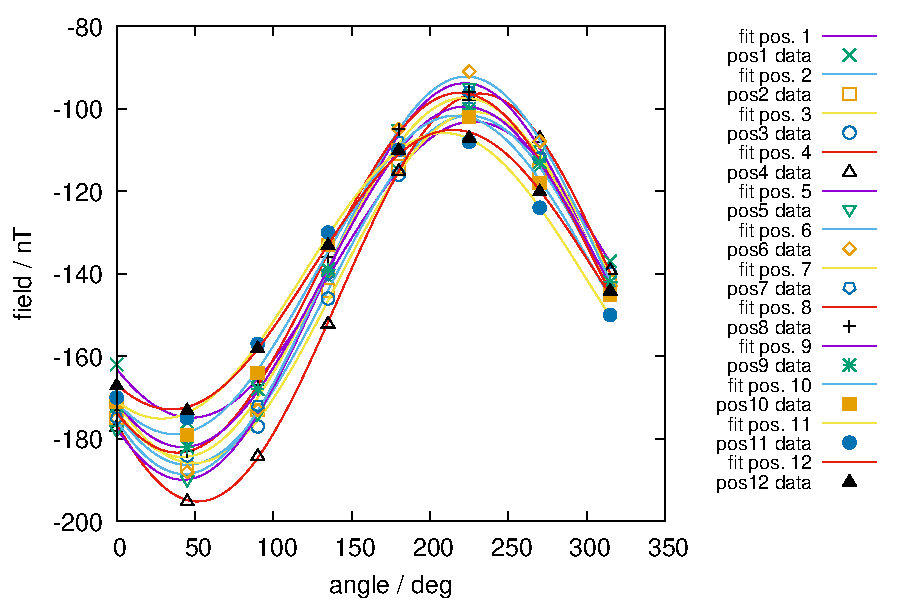
\includegraphics[width=0.99\textwidth]{/figures/experiments/fluxgate/yField.pdf}
            \caption[Calibration results X/Y]{Calibration data of X- and Y-fluxgate sensor. Each dataset corresponds to a full rotation of the fluxgate device around the z axis at one position inside the MuMetal shield. The solid lines correspond to a sine fit to each dataset with phase, amplitude and offset as fitting parameters. Error bars are not
                \label{fig:results:fluxgate:xysinus}
            displayed for better visibility.}
        \end{figure}
        The fit parameters shown in table \ref{table:results:calibrationFitParams} allow for calibration of X- and Y- channel by calculating the average offset for all positions.
        \begin{table}
            \centering
            \begin{tabular}{|r|ccccccc|}
                \hline
                position & 1& 2 & 3 & 4 & 5 & 6 & 7 \\
                \hline 
                amplitude x& 12.4 & 22.4 & 27.0 & 35.9 & 39.6 & 45.2 & 42.5\\
                offset x&    5.25 & -0.50 & 0.62 & -0.87 & -3.37 & 1.12 & 0.75 \\
                phase x&    -0.55 & -0.63 & -0.74 & -0.87 & -0.66 & -0.76 & -0.76 \\

                \hline
                position & 8 & 9 & 10 & 11 & 12 &&\\
                \hline
                amplitude x & 42.9 & 45.1 & 45.4 & 44.6 & 40.6 && \\
                offset x & 1.0 &  0.62 & 0.63 & 2.99 & 2.24 && \\
                phase x & -0.74 & -0.84 & -0.73 & -0.62 & -0.64&&  \\
                \hline
                position & 1& 2 & 3 & 4 & 5 & 6 & 7\\
                \hline
                amplitude y & 35.8 & 42.2 & 42.5 & 49.4 & 48.0 & 48.1 & 43.5 \\
                offset y & -139.0 & -144.0 & -143.37 & -145.75 & -141.88 & -140.38 & -140.88 \\
                phase y & 0.73 & 0.78 & 0.71 & 0.66 & 0.83 & 0.81 & 0.83 \\
                \hline
                position &  8 & 9 & 10 & 11 & 12&&\\
                \hline
                amplitude y & 43.5 & 41.2 & 38.5 & 34.5 & 33.8 &&\\
                offset y & -139.75 & -140.75 & -140.25 & -140.5 & -139.0 &&\\
                phase y & 0.89 & 0.83 & 0.93 & 1.07 & 0.96 && \\
                \hline
            \end{tabular}
            \caption[Fluxgate calibration results]{Calibration results at different positions of the fluxgate inside the mu metal shield. See figure \ref{fig:results:fluxgate:plotSpatial} for a comprehensive visualization of those results. Figure \ref{fig:matMeth:shields15N} shows the dimensions and positions of the setup.}
            \label{table:results:calibrationFitParams}
        \end{table}
        \begin{figure}
            \centering
            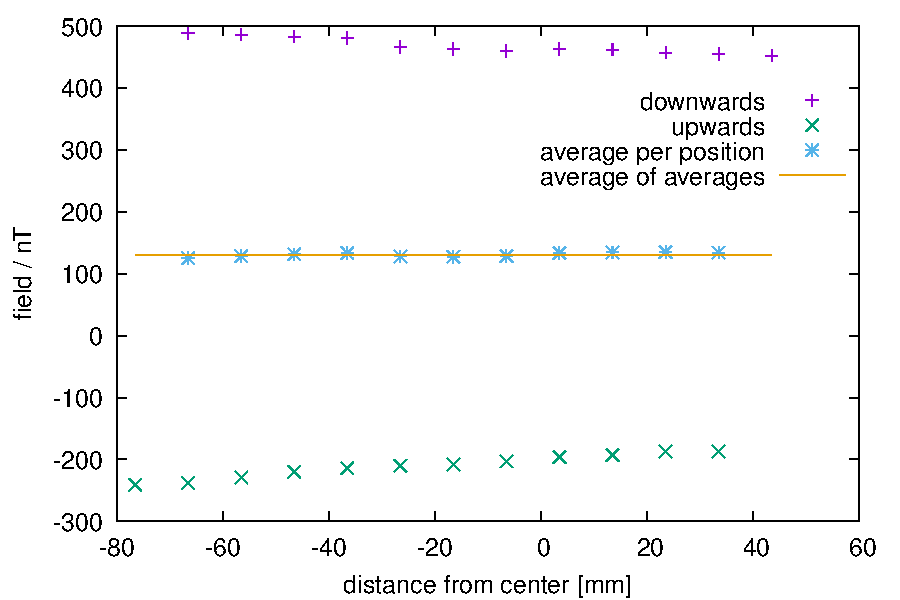
\includegraphics[width=0.99\textwidth]{/figures/experiments/fluxgate/zField.pdf}
            \caption[calibration results Z]{Calibration of the Z-channel. Due to spatial limitations, no full rotation in z direction was possible. The two datasets represent one measurement in "upwards" and one in "downwards" direction. The solid line represents the average of the positional averages of the two directions.}
            \label{fig:results:fluxgate:zcal}
        \end{figure}
        Using the data for calibration, the measurements of the X- and Y-channels can be used to plot a 2D-section of the field using the phase of the fit as the field direction and the amplitude as its magnitude. Both X- and Y-sensor are shown in figure \ref{fig:results:fluxgate:plotSpatial}. The absolute positions are indicated in the figure to enable comparison of the individual results in the same absolute position. The same data is also shown in a 3D plot (fig. \ref{fig:results:fluxgate:plotSpatial}) to show the field progression inside the mu metal shield. The calibration of the z channel (using only up- and down-direction, see section \ref{sec:matMeth:fluxgateMeasurementPrinciple}) is shown in figure \ref{fig:results:fluxgate:zcal}.
        \begin{figure}
            \centering
            %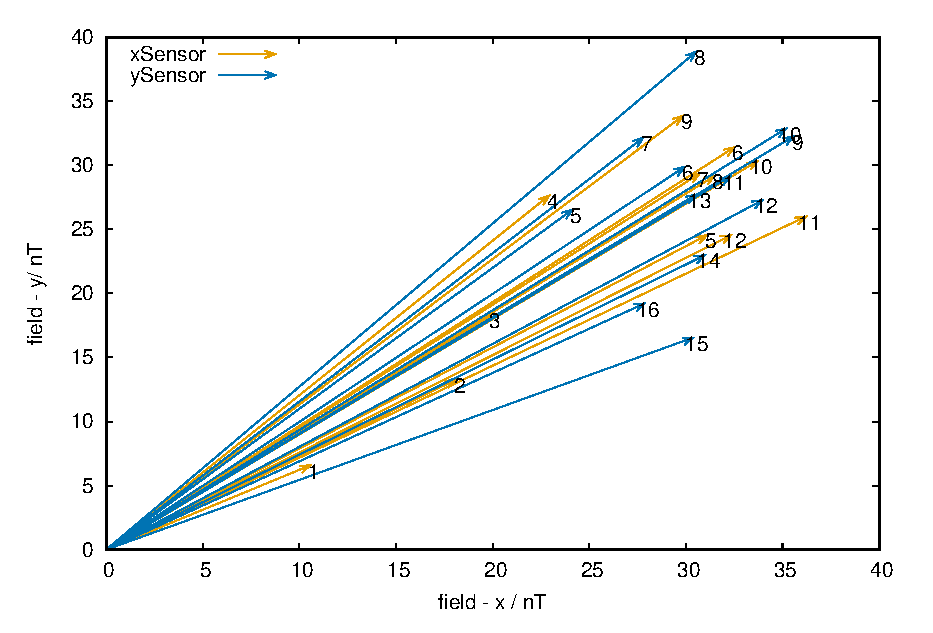
\includegraphics{/home/philipp/Documents/thesis/figures/experiments/fluxgate/spatial2dProjection.eps}
            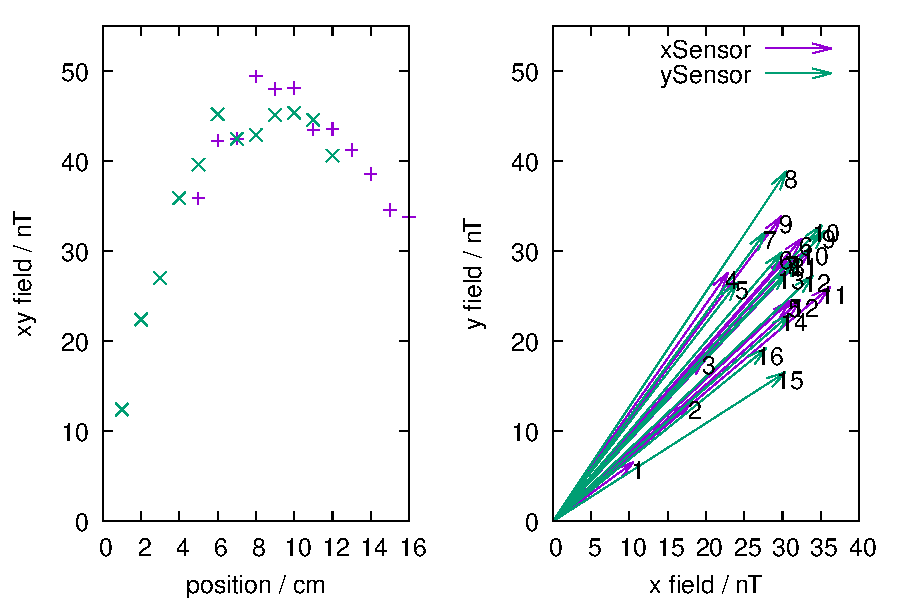
\includegraphics{/figures/experiments/fluxgate/spatial2dProjection.pdf}
            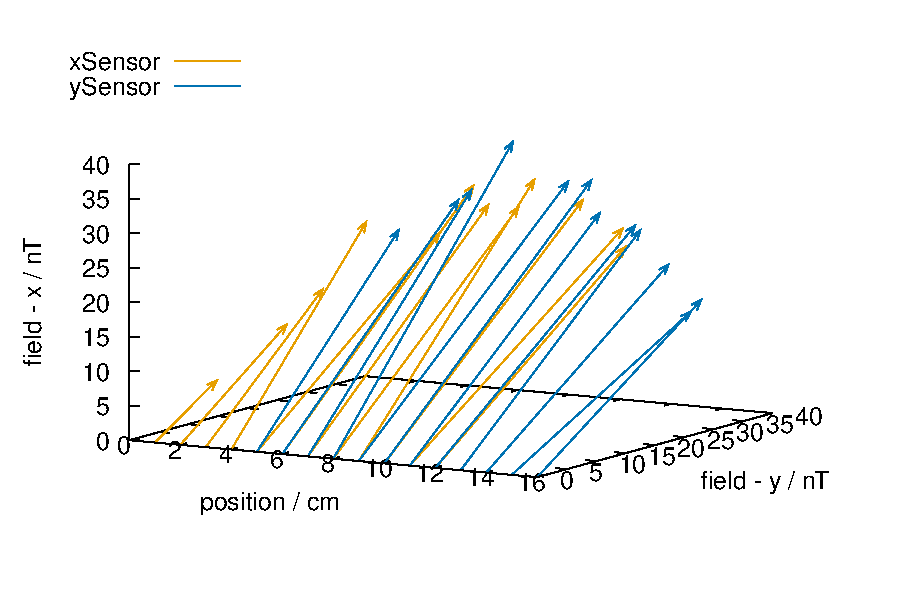
\includegraphics{/figures/experiments/fluxgate/spatial3d.pdf}
            \caption[Fluxgate calibration]{Results of the fluxgate calibration visualized: on top, the two projected views are shown that visualize the absolute field values in the x-y-plane (left) and the field's direction (right). In the right plot, the numbers inside the graph correspond to the positions listed in table \ref{table:results:calibrationFitParams}. The field reaches a maximum in the center of the shield at around \SI{8}{\centi\meter}. The angle of the field remains fairly constant within an angle of $\approx$ \SI{30}{\degree}. In the lower part, the same data is shown as a 3d plot for a better overview.}
            \label{fig:results:fluxgate:plotSpatial}
        \end{figure}
\section{Measurements}
    \subsection{Low field NMR}
    \label{chap:results:lowFieldNMR}
    The low field NMR was used for hyperpolarization experiments as well as thermal measurements. Low field spectra were acquired using different hardware in the modular setup. The main difference between setups was the exchanged $B_0$ coil. The initially used solenoid coil showed linewidths of about 0.5 - \SI{1}{\kilo\hertz}. Due to mechanical destruction of one coil and those rather wide lines, a new coil design was simulated and built (for simulation results, see figure \ref{fig:results:compensationWindOptimization}) using Biot Savart calculations. While currents to generate the same field were higher by a factor of about 2, field homogeneity improved greatly and now shows linewidths of about \SI{21}{\hertz} (figure \ref{results:lowFieldSpectrometer:thinLine}) which is an improvement of about a factor of 24. Flip angle calibrations for different pulse durations were calibrated and yielded the results shown in table \ref{table:results:FA}. These results were used in successive measurements with the low field NMR unless stated differently.
        \begin{table}
            \centering
            \begin{tabular}{|c|cccc|}
            \hline
            pulse duration / $\mu$s & 500 & 700 &  800 & 1500 \\
            \hline
            $\mathrm{V}_{\SI{90}{\degree}}$ / V & 5.8 & 4.5 &  2.1&  0.75 \\
            \hline
            \end{tabular} 
            \caption[Flip angle calibration results]{Results of the manual flip angle calibration of the saddle excitation coil using the syringe receive coil for pulse durations ranging from 500 to 1500 ms and block pulse shape. Note that the factors of voltage and pulse duration do not scale inversely as would be expected (see equation \ref{eq:theory:FA}).}
            \label{table:results:FA}
        \end{table}
            \begin{figure}
                \centering
                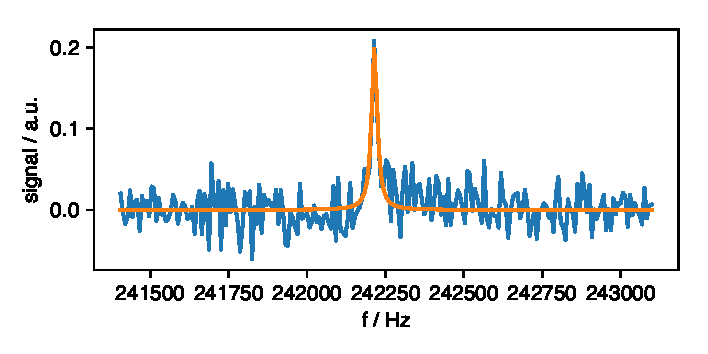
\includegraphics[width = 0.99\textwidth]{/figures/experiments/lowFieldSpectrometer/helmholtzNarrowLine.pdf}
                \caption[Thin line helmholtz coils]{A $_1\mathrm{H}$ line of a Magnevist doped water sample inside the 'syringe coil'. Linewidth is down to \SI{21}{\hertz} in this example without the use of shim coils.}
                \label{results:lowFieldSpectrometer:thinLine}
            \end{figure}
    \subsection{Sabre in water}
    The hyperpolarization experiments in the low field spectrometer were moved from non-biocompatible methanol as the solvent and pyridine as the substrate to nicotinamide (vitamin B$_3$) in D$_2$O. For measurements of continuously hyperpolarized nicotinamide in deuterated water, the buildup of hyperpolarization was observed as a function of the delay between individual measurements (TR). Here, TR was varied from \SI{1}{\second} to \SI{30}{\second}, the signal was stronger for longer TR because this allowed for a longer buildup of hyperpolarized molecules before readout of the signal. The difference between TR~=~\SI{15}{\second} and TR~=~\SI{30}{\second} is already within the margin of error and implies that a plateau is reached in this domain which can be easily explained by considering that the buildup of hyperpolarization is counteracted by T$_1$ relaxation back to thermal equilibrium. Note that a dummy scan was necessary for each TR measurement series to deplete the previously built hyperpolarization. The effective buildup rate can be calculated from these results (table \ref{table:results:TRvariation}) and is shown in figure \ref{fig:results:lowFieldSpectrometer:TRvariation}. Using this data, the specific buildup rate, i.e. an effective T$_1$ was determined to be \SI{5.4\pm 0.2}{\second} for D2O. Similarly, for $\mathrm{H}_2\mathrm{O}$, a lower T$_1$ of \SI{2.4\pm0.2}{\second} was found. Both measurements were carried out at a magnetic field of \SI{5}{\milli\tesla}.
        \begin{table}
            \centering
            \begin{tabular}{|c|ccccccccc|}
                \hline
                TR [s] & 1 & 2 & 3 & 4 & 6 & 8 & 10 & 15 & 30 \\
                \hline
                signal [a.u] & 1.62 & 4.19 & 6.03 & 8.10 & 11.03 & 12.89 & 14.29 & 16.29 & 16.84\\
                stdev [a.u.] & 0.61 & 0.56 & 0.59 & 0.52 & 0.50 & 0.50& 0.52 & 0.51 & 0.53\\
                \hline
            \end{tabular}
            \caption[TR-variation results]{Average signal of each TR measurement series excluding the dummy scan destroying previously accumulated polarization. Standard deviation is additionally given.}
            \label{table:results:TRvariation}
        \end{table}
        \begin{figure}
            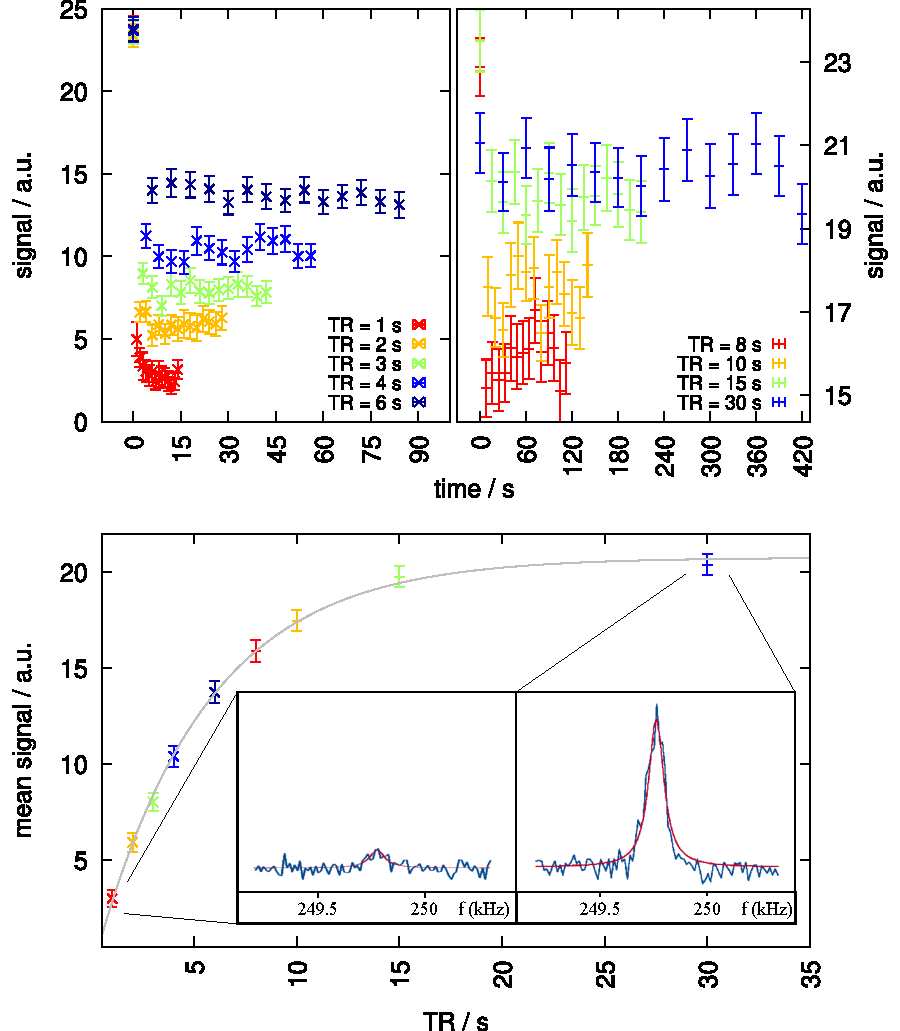
\includegraphics[width=0.99\textwidth]{/figures/experiments/lowFieldSpectrometer/inSituSabreWater/combinedInsert.pdf}
            \caption[TR variation]{Variation of the TR in the measurements of a continuously hyperpolarized sample of Ir-IMes and nicotinamide in D$_2$O. Each TR was measured 10 times, resulting in varying cumulative measurement times. Note that one 'dummy scan' was necessary to reach the steady state for each TR, to be seen at timepoint 0. Average values increase with TR and correspondingly longer buildup rates. Bottom: The average values excluding the first measurement for every TR, which is not yet in the steady state equilibrium, over TR. An exponential function was fit to the data revealing a buildup rate, i.e. an effective T$_1$ of \SI{5.4\pm 0.2}{\second}}
            \label{fig:results:lowFieldSpectrometer:TRvariation}
        \end{figure}
        The maximum polarization achieved for nicotinamide in D2O in this setup was $4.6\cdot 10^{-5}\si{\percent}$.
    \subsection{Imaging of continuously hyperpolarized solution}
    It was further demonstrated that imaging of the hyperpolarized solution is possible and effective.
    Using the Magritek Terranova (section \ref{sec:matMeth:magritek}), images of continuously hyperpolarized solutions were acquired. Using watery SABRE solutions, imaging at low fields, specifically even at earth magnetic field, were possible. Prior to imaging, a prepolarization field or, in this case, a hyperpolarization field of $\approx$ \SI{5}{\milli\tesla} was used. The results of such an image at Earth's magnetic field is shown in figure \ref{fig:results:earthFieldImage}.  The SNR of the much more lowly concentrated nicotinamide (\SI{1.3}{\milli\Molar}, corresponding to \SI{12}{\milli\gram} nicotinamide in \SI{5}{\milli\litre} D2O) was higher than that of a highly concentrated water sample (\SI{20}{\milli\litre} of \SI{55}{\Molar} water) with a much larger volume and relaxation doping to enable fast imaging by reducing T1. The latter showed a SNR of 4.7. For the image, a calculated signal increase of 9500 corresponding to a polarization of $1.5\cdot 10^{-4}$ was achieved.
    \begin{figure}
            \includegraphics[width=0.9\textwidth]{/figures/experiments/earthFieldImaging/2dImagePlusOutline}
            \caption[Earth field SABRE image]{An image of a continuously hyperpolarized sample and a Gadolinium doped water reference acquired at earth magnetic field after prepolarization for \SI{30}{\second}. The much lower concentrated nicotinamide sample (\SI{1.3}{\milli\Molar}) shows higher signal than the thermally polarized water (\SI{55}{\Molar}), though water is also prepolarized at \SI{5}{\milli\tesla}. Resolution is (\SI{1.6}{\milli\meter})$^2$ with an acquisition time of \SI{5}{\minute} \SI{20}{\second}.}
            \label{fig:results:earthFieldImage}
        \end{figure}
        Linewidths in single shot experiments after shimming were in the \SI{1}{\hertz} range and thus more narrow than the low field spectrometer's lines of a similar sample. 
        %Considering the by a factor 100 lower Earth's magnetic field, the relative homogeneity of the Low field spectrometer was comparable (even slightly better) though.
    \subsection{Sabre in cell solution and blood}
    Measurements in pure water yielded sufficient signal to try using substances as solvents that have a direct biological relevance. Dulbecco's Phosphate Buffered Saline cell culture solution (DPBS) was the first step forward and unfortunately showed to already significantly reduce the polarization yield. Addition of \SI{0.5}{\milli\litre} of DPBS reduced the signal by a factor of 3. This already indicated that with human blood as an addition to the solution, the performance would not be better if not worse. Measurements confirmed this suspicion, the signal showed to already drop by a factor of \~8 after injection of 0.3 ml of human blood into the solution. Adding \SI{0.5}{\milli\litre} of blood completely eliminates the signal. SNR of these measurements was low compared to other hyperpolarized solutions. That may indicate that in case of a better base solution, som residual signal might have been left (compare section \ref{sec:discussion:cellSolution}).
        \begin{figure}
            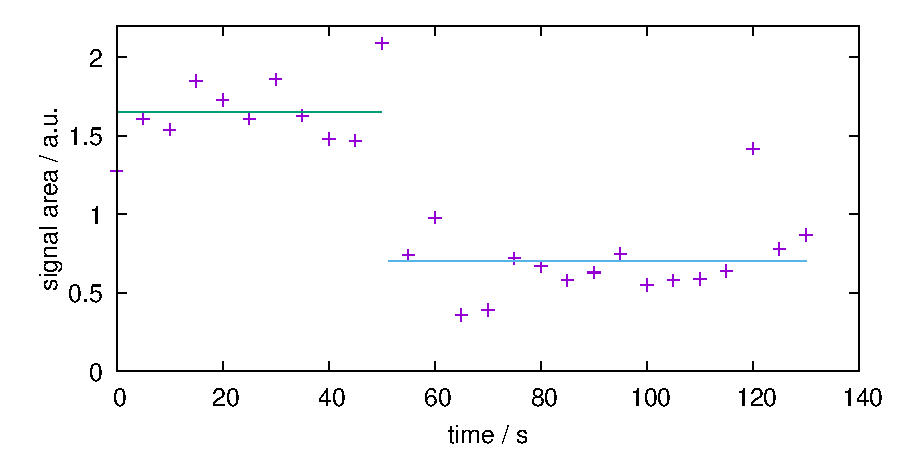
\includegraphics[width=0.99\textwidth]{/figures/experiments/lowFieldSpectrometer/inSituSabreWater/timeSeriesCellCultureSolution.pdf}
            \caption[Cell culture solution addition to hyperpolarized signal]{Time course of the signal intensity (peak height) when adding cell culture solution to a continuously hyperpolarized solution of \SI{3}{\milli\gram} IrIMes, \SI{12}{\milli\gram} of nicotinamide in \SI{3}{\milli\litre} D2O. Note the strong signal drop after addition of \SI{0.5}{\milli\litre} of cell culture solution to the sample at t=\SI{50}{\second}. The straight and dashed lines indicate the average before and after addition.}
            \label{chap:MaterialsAndMethods:bloodInjection}
        \end{figure}
        \begin{figure}
            \centering
            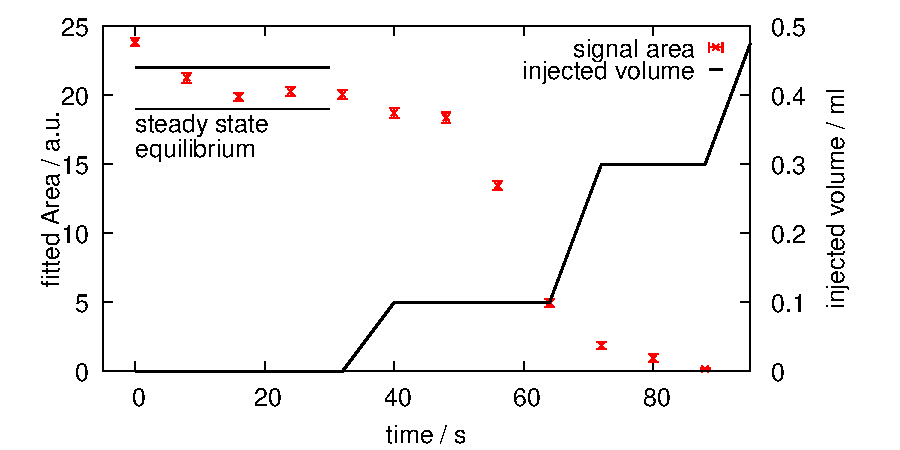
\includegraphics[width=0.99\textwidth]{/figures/experiments/lowFieldSpectrometer/inSituSabreWater/signalVariation.pdf}
            \caption[Blood addition to hyperpolarized signal]{Signal drop during the injection of \SI{0.5}{\milli\liter} of blood into the solution providing hyperpolarized signal which was continuously generated by steadily bubbling fresh pH$_2$ through the solution. First measurements show a slight drop until a steady state is reached. The steady state then loses signal intensity as the amount of substance injected is increased.}
            \label{chap:MaterialsAndMethods:bloodInjection2}
        \end{figure}
    \subsection{Liposomes and SABRE}
    \label{sec:results:liposomes}
    The results of cell culture solution and human blood addition to a working, hyperpolarized sample suggested that other approaches were necessary to achieve hyperpolarization in biologically relevant surroundings. The previously described method of encapsulation of substrate and catalyst in double layered liposomes (section \ref{sec:matMeth:liposomes}) was used. With methanol and pyridine, the formation of the liposomes was hindered which made those unsuitable. While the liposomes formed with the materials described in the materials section, the size distribution according to the lipochemists was broader than usual. The experiments trying to hyperpolarize the liposomal structures failed and it showed that the addition of the components used in the generation of liposomes into a working hyperpolarized solution already depleted the signal to a non-detectable level. Different solvents and substrates were tested in combinations but did not yield any observable signal.  
\subsection{$^{15}$N SABRE}
As the in-vivo application of continuous hyperpolarization showed to be limited, a high batch polarization (high here meaning in the 1-10 percent range) was consequently pursued to serve as indicators of metabolic processes or other factors such as pH values.
        $^{15}\mathrm{N}$ labeled substances were used to generate high polarization on the substrate in \si{\nano\tesla} fields. Results are shown here and include spectroscopic as well as imaging experiments.
    \subsubsection{$\mathrm{T_1}$ and $\mathrm{T_2}$ measurements}
    The relaxation times of the sample are relevant to subsequent measurements of spectra and images and were measured for both 15N-Glycine phantom and a neat, thermally polarized 15N-Pyridine sample.
    Results for T$_1$ measurements are shown in figure \ref{fig:results:T1T2}. Fit parameters are given in table \ref{table:results:T1T2}. For \SI{12}{\micro\litre} $^{15}$N pyridine and \SI{4}{\milli\gram} Ir-Imes catalyst dissolve in the sample$\mathrm{T}_1$ was found to be \SI{52.6\pm 2.7}{\second} for MeOH as a solvent and \SI{76.9\pm 5.6}{\second} for MeOD. $\mathrm{T}_2$ for the same sample was measured to be \SI{435\pm 38}{\milli\second}.
        \begin{table}
            \begin{tabular}{|c|c|c|}
                \hline
                    & time constant / s & error / s\\
                    \hline
                $\mathrm{T_1}$ MeOH & 52.6 & 2.7  \\
                $\mathrm{T_1}$ MeOD & 76.9 & 5.9  \\
                $\mathrm{T_2}$ MeOD &  0.435 & 0.038 \\
                glycine phantom $\mathrm{T_1}$& \SI{65.5}{\milli\second}&  \\
                glycine phantom $\mathrm{T_2}$&\SI{20.4}{\milli\second} &  \\
                \hline
            \end{tabular}
            \caption[Relaxation times]{Relaxation times T$_1$ and $T_2$ of 15N-labeled pyridine. MeOD as a solvent increases T$_1$ slightly and was used for subsequent measurements.\todo{fill in values}}
            \label{table:results:T1T2}
        \end{table}
        \begin{figure}
            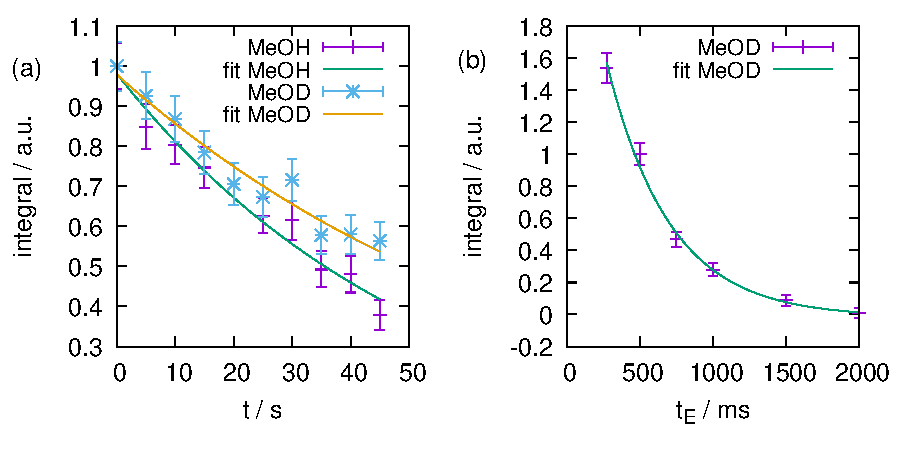
\includegraphics[width = 0.99\textwidth]{/figures/experiments/15NSabre/relaxation/T1_T2.pdf}
            \caption[T1/T2 of 15N]{$T_1$and $T_2$ relaxation times for a hyperpolarized pyridine sample. T$_1$ was measured in MeOH and MeOD. Both solvents show similar relaxation times while the deuterated solvent's is slightly longer. $T_2$ is significantly shorter than $T_1$.}
            \label{fig:results:T1T2}
        \end{figure}
        The shorter relaxation times of the Glycine phantom allow to run adjustments quickly as the long T$_1$ of 15N-pyridine in combination with its low concentration in the hyperpolarization samples would make running scanner adjustments impossible.
    \subsubsection{Pressure dependence}
    To investigate the influence of the pH$_2$ pressure during bubbling, the hyperpolarization experiment was repeated multiple times at different pressures. The results of these measurements are shown in figure \ref{fig:results:15N:pressureDependence}. A mostly linear pressure dependence can be estimated from the data indicating that the catalytic reaction is still in the low concentration regime of hydrogen dissolved in solution.
        \begin{figure}
            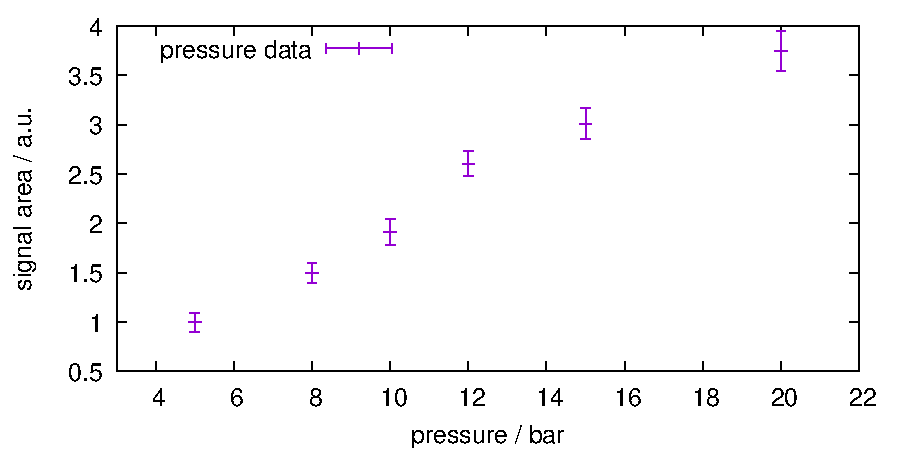
\includegraphics[width = 0.99\textwidth]{/figures/experiments/15NSabre/pressureDependence/pressureDependence.pdf}
            \caption[Pressure dependence]{Signal area of integrals at different parahydrogen pressures used for polarization. Higher pressures lead to higher signal over the pressure range shown here. A linear behavior can be estimated from the data in the range provided.}
            \label{fig:results:15N:pressureDependence}
        \end{figure}
    \subsubsection{Concentration dependence}
        The absolute concentrations of the SABRE components as well as their relative concentration have an influence on the overall signal, i.e. magnetization of the sample. Here, the concentration of pyridine is lowered over the course of the measurements by diluting the sample while the concentration of the catalyst is kept constant. The signal of the solution increases over the course of the measurements. That means that falling concentration but at constant amount of substance for $^{15}$N-pyridine, the polarization increased.
        \begin{figure}
            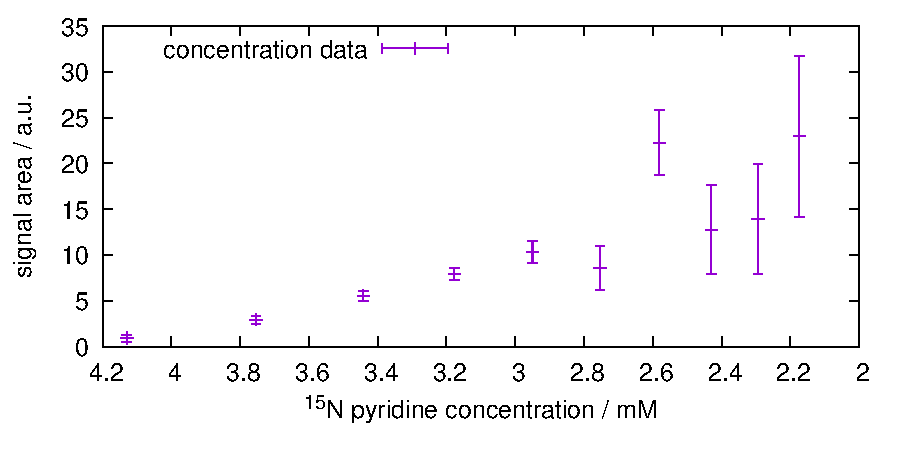
\includegraphics[width=0.99\textwidth]{/figures/experiments/15NSabre/concentrationDependence/concentrationDependence.pdf}
            \caption[Concentration dependence]{The signal of a solution of IrIMes and $^{15}$N pyridine that is diluted from left to right by dilution with a solvent-catalyst mixture of the same concentration used in the sample. Concentration of catalyst is thus constant throughout the measurement. Signal rises with rising dilution, i.e. with lower concentration.}
            \label{fig:results:15N:concentrationDependence}
        \end{figure}
    \subsubsection{Flow dependence}
    Similar to pressures, flow rates have been varied to estimate their effect on the reaction's efficiency. In contrast to pressure, flow was not linearly correlated to signal intensity. As different flow rates change the bubble sizes as well as the number of flow channels forming inside the solution starting from the bottom plate of the reactor (see figure \ref{figure:materialsMethods:probesPSU}), a more complex behaviour is expected and shown in figure \ref{fig:results:15N:flowDependence}. Two pressures are shown for different flow rates set at the needle valve. For both pressures, the higher flows cause higher signal up to a certain point. At \SI{10}{\bar} signal remains at constant levels from \SI{5}{\litre\per\hour}, for \SI{20}{\bar}, from a flow setting of \SI{4}{\litre\per\hour} the same effect is observable. This can be explained by the saturation of solution that sets in at different flows for different pressures, depending on the geometric reality of the flowing gas. Therefore, the saturation of the solution with parahydrogen gas is reached at lower flows  of \SI{4}{\liter\per\hour} for the higher pressure of \SI{20}{\bar}, where the overall signal of the plateau is higher than for the low pressure of \SI{10}{\bar} where a flow of \SI{6}{\liter\per\hour} is required to maximize the signal.
        \begin{figure}
            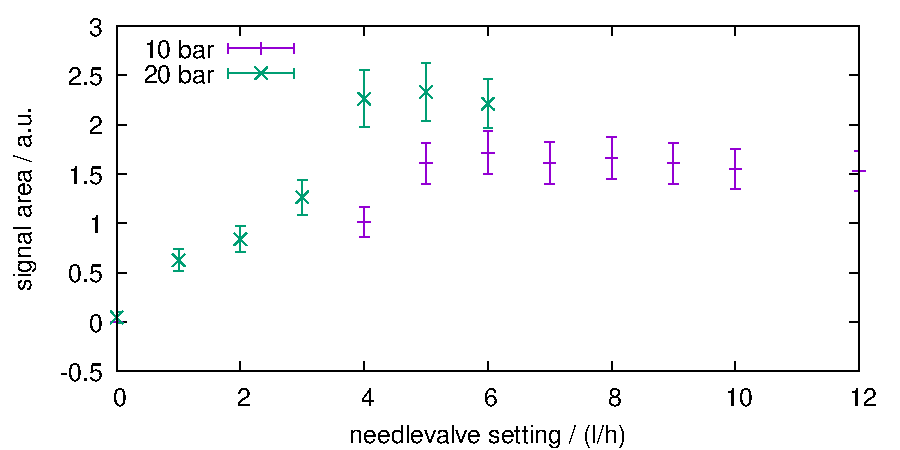
\includegraphics[width=0.99\textwidth]{/figures/experiments/15NSabre/flowDependence/flowDependence.pdf}
            \caption[Flow dependence]{The signal depending on the flow of parahydrogen through the sample at nanotesla fields. \SI{10}{\bar} and \SI{20}{\bar} pressure were measured at different needle valve settings. Higher flows first lead to higher signal, but note the flattening of the signal at high flows for both pressures.}
            \label{fig:results:15N:flowDependence}
        \end{figure}
    \subsection{Magnetic field dependence}
    Magnetic field dependence of the polarization was measured by adjusting the field using the solenoid coil and dual Helmholtz pair mounted inside the MuMetal shields. The currents necessary for optimum fields were a function of the residual magnetization of the shield. Measurements of polarization and current-field correlation were conducted separately. Figure \ref{fig:results:15N:fieldDependence} shows the signal for different polarization fields inside the shield. The result shows that the field reduction generated by the shielding is large enough to undercut the optimal polarization fields as the signal drops between the two maxima that show up for both coils: In case of the solenoid coil for \SI{-120}{\nano\tesla} and \SI{-280}{\nano\tesla} and in case of the Helmholtz assembly for \SI{-100}{\nano\tesla} and \SI{20}{\nano\tesla}. To generate maximum signal, one of the fields generating maximum signal is used in the measurements.
        \begin{figure}
            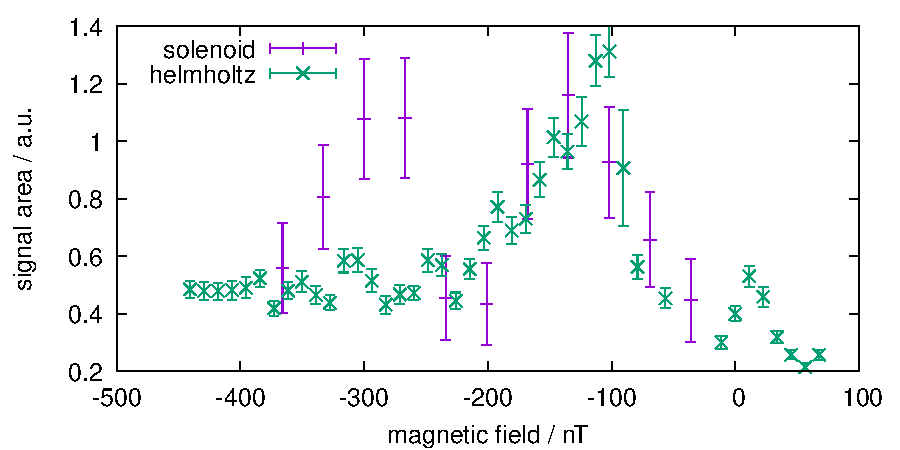
\includegraphics[width=0.99\textwidth]{/figures/experiments/15NSabre/fieldDependence/fieldDependenceCombined.pdf}
            \caption[Magnetic field dependence]{Signal over polarization field for both the solenoid coil and the Helmholtz coil  assembly. Both coil setups  show distinct peaks at slightly different field strengths, the symmetry axis for the Helmholtz coils is at around \SI{-30}{\nano\tesla} whereas it is around \SI{-210}{\nano\tesla} for the Helmholtz assembly.}
            \label{fig:results:15N:fieldDependence}
        \end{figure}
    \subsection{Polarization measurements}
    The scheme used in the first, preliminary tests provided polarizations in the range of \SI{0.1}{\percent}. This value was drastically improved by using a more sophisticated approach, i.e. an automated high pressure shuttling system to generate high polarizations reproducibly and even at high concentrations to generate high magnetization.
    Polarizations in high concentration regimes and under otherwise optimal parameters (i.e. high flow of \SI{6}{\litre\per\minute}, high pressures of \SI{50}{\bar} and a field of \SI{120}{\nano\tesla}) the maximum polarization measured was $\mathrm{P} = 3.9\% \pm 0.2 \%$. The parameter that was not adaptively controlled in this setup, but does have a substantial influence on the magnetization yield was the temperature of the sample.  It decreased when parahydrogen flowed through the volatile methanol used as solvent, see \ref{cd:sabreShuttling:tempControl} for a closer discussion.
    Two methods were used for quantification - comparison of the hyperpolarized signal to thermal NMR signal of the same sample, as a very reliable, but slow method, and comparison to the $^{15}$N glycine phantom's NMR signal which is less reliable per se but fast. Both methods yield similar results if match and tune of the $^{15}$N coil are readjusted after exchanging the sample for the phantom. This ensures a similar flip angle used in the phantom measurement and thus a decent estimate of polarization. Figure \ref{fig:results:15N:polarization} shows the results of these measurements.
        \begin{figure}
            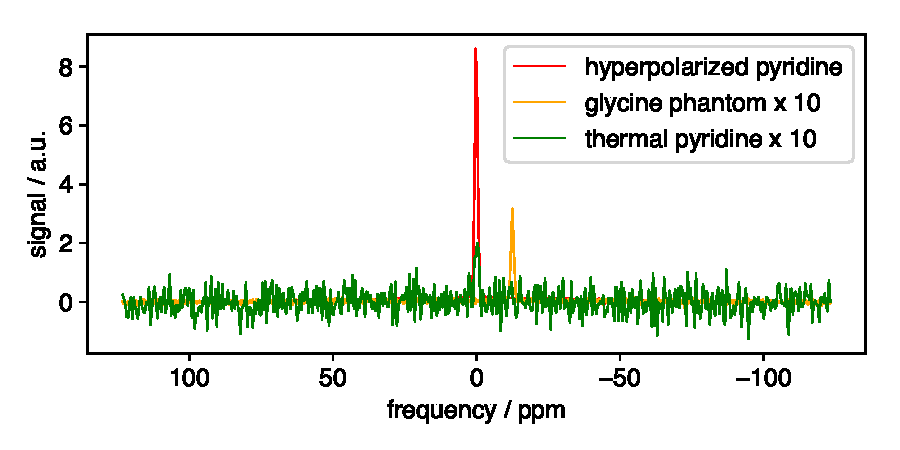
\includegraphics[width=0.99\textwidth]{/figures/experiments/15NSabre/polarization/highPolarization.pdf}
            \caption[High $^{15}$N polarization]{15N spectra of the hyperpolarized $^{15}$N pyridine sample, the sample in its thermal state and the $^{15}$N glycine phantom. Note the frequency shift due to the different chemical shift properties of the two molecules. The relative signal intensity of the hyperpolarized sample is 38.2, additionally, the thermal signal was averaged 250 times. Note the high noise levels on the thermal measurement due to signal averaging.}
            \label{fig:results:15N:polarization}
        \end{figure}
        \subsection{15N imaging}
        By optimization of the parameters above, a signal increase of about a factor of 15 was achieved. Preliminary images of a NMR tube filled with hyperpolarizable solution and more highly resolved images using the setup sonstructed and built in this work are shown in figure \ref{fig:results:15Nimage}.
        \begin{figure}
            \includegraphics[width=0.9\textwidth]{/figures/experiments/15NSabre/badGoodImage.pdf}
            \caption[15N image]{Images of $^{15}$N hyperpolarized pyridine. The laft image is recorded in a preliminary setup without optimized parameters. The right image was recorded after optimization of setup and parameters.}
            \label{fig:results:15Nimage}

        \end{figure}
\section{Simulations}
        \label{sec:results:sim}
        \subsection{Static magnetic field calculations}
        \label{sec:results:sim:B0}
            Using Biot Savart's law, a Matlab program to calculate the fields of current carrying conductors was implemented. Structural elements were mostly solenoids, but also saddle and Helmholtz coils were considered and can easily be implemented.
            \subsubsection{Solenoid Coil}
            \label{sec:results:B0solenoid}
            The magnetic field of the primary B0 coil used in the low field NMR system (see section \ref{sec:matMeth:lowFieldSpectrometer}) was calculated and the length of the compensation windings was optimized for field homogeneity.
                \begin{figure}
                    \centering
                    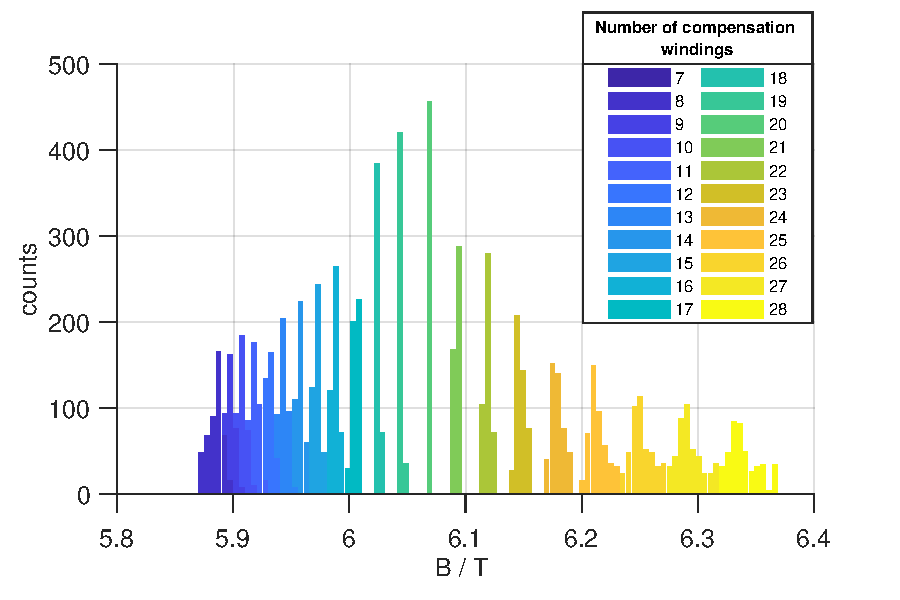
\includegraphics[width=0.99\textwidth]{/figures/simulations/B0/solenoidCoil/compensationWinds.pdf}
                    \caption[Compensation wind optimization]{Histograms of the magnetic field strength. Each voxel's field inside the ROI is calculated and binned. From left to right, number of compensation windings rise. This leads to a field increase and change in homogeneity. Central winding numbers are the most homogeneous ones discovered.}
                    \label{fig:results:compensationWindOptimization}
                \end{figure}
            It can be seen that different numbers of turns for the optimization windings change both the overall field strength (simple superposition) and its homogeneity. a rough binning was chosen at first to easily discover the overall region of high homogeneity and then refined to streamline homogeneity in this region.
            Figure \ref{fig:results:compensationWindOptimization} furthermore portraits the rather substantial influence of a single wind indicating that the manufacturing process must be well controlled while the variation is limited by the integer number of winding necessary to keep the fields rotational symmetry.
            The  overall magnetic field strength the coil generates in the optimized case is plotted in figure \ref{fig:results:solenoidField} in a plane parallel to the magnetic fields main direction. Despite the simulations considering to solenoidal character of the coil, rotation of the plane around the magnetic field's main axis did not affect homogeneity greatly. The overall shape of the field histogram is not a Lorentzian; this confirms what was found experimentally for the rather wide peaks (> \SI{100}{\hertz} linewidth) fitted with Lorentzian that showed poor resemblance to the Lorentzian distribution. Figure \ref{fig:results:solenoidField} shows an exemplary result of the optimization in a more global view. Both the pure solenoids magnetic field distribution and that of the compensation windings is shown, their combined field shows a flat field distribution in the central volume of 3x3x3 \si{\cm\cubed} (only two dimensions displayed).
            \begin{figure}
                \includegraphics[width=0.99\textwidth]{/figures/simulations/B0/solenoidCoil/solenoidNoCompFull.pdf}
                \includegraphics[width=0.99\textwidth]{/figures/simulations/B0/solenoidCoil/compensationWindsOnly.pdf}
                \includegraphics[width=0.99\textwidth]{/figures/simulations/B0/solenoidCoil/compensationWindsFull.pdf}
                \caption[Solenoid and compensation field]{The magnetic field generated by a pure solenoid, that of the compensation windings optimized for that solenoid and their combined fields from top to bottom. Note the concave curvature of the central, relevant region for the compensation windings that homogenize the convex curvature of the pure solenoid. The relative spread in the central \SI{3}{\cm} sphere is about $10^{-3}$ }
                \label{fig:results:solenoidField}
            \end{figure}
        \subsubsection{Helmholtz Array}
        The previously described Biot Savart simulation was used again to simulate the field of the Helmholtz array later utilized in the experiments. The simulations were used to optimize the parameters for the setup before manufacture. Simulation steps for the distance between the two Helmholtz pairs are shown in figure \ref{fig:results:optimizationSteps}.
        \begin{figure}
            \centering
            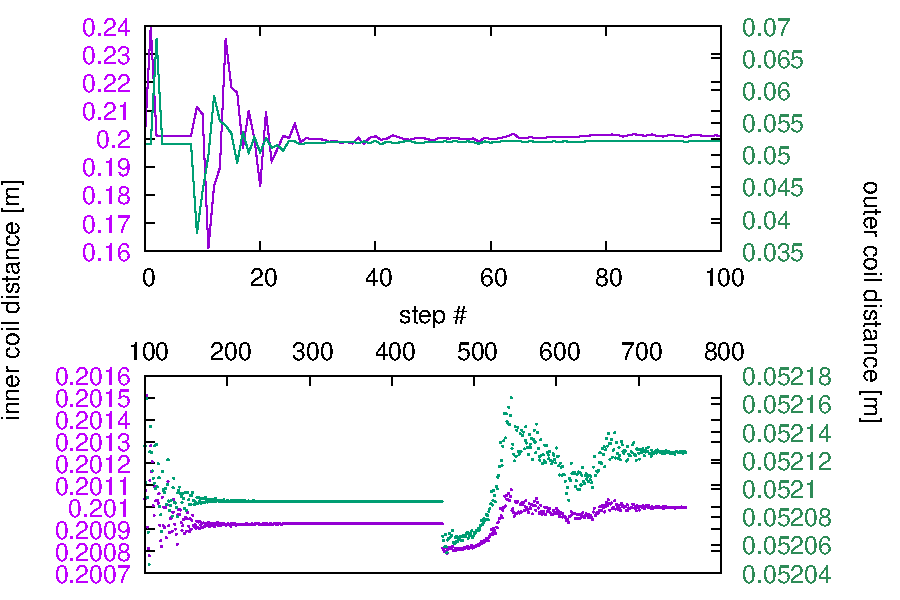
\includegraphics[width=0.99\textwidth]{/figures/simulations/B0/helmholtzCoil/optimizationSteps.pdf}
            \caption[Helmholtz coil optimization]{Optimization steps of the two distances of inner and outer coil pair. Note the small range in the lower graph that is probably already inside the margin of error of manufacture and actual positioning.}
            \label{fig:results:optimizationSteps}
        \end{figure}
        Note that the figures shown here do not include the optimization of the current ratio between the two coil pairs. The simulation results concerning the positions of the coils are shown in figure \ref{fig:results:distanceVariation}. A closeup of the central region is plotted in figure \ref{fig:results:fieldSpread}. The optimal result lies in the central grove marked in a bright yellow. Comparing the field spreads shown in figure \ref{fig:results:fieldSpread} to the central field in figure \ref{fig:results:solenoidField} shows a factor $\sim 50$ improvement.
        \begin{figure}
           \centering
           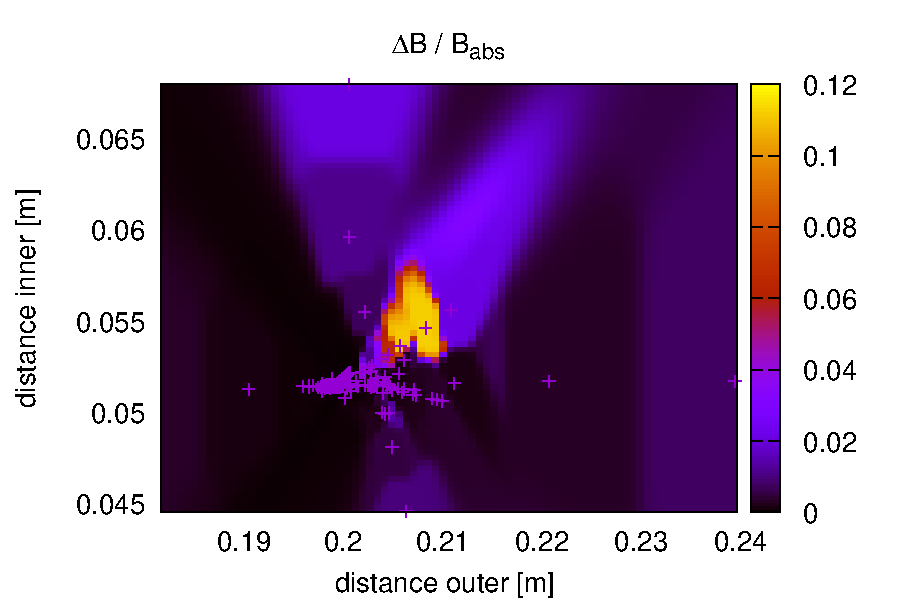
\includegraphics[width = \textwidth]{/figures/simulations/B0/helmholtzCoil/distanceVariation.pdf}
           \caption[Optimization steps]{Optimization of the coils distances by 'fminsearchbnd'. Note that the current ratio of the coils was also varied in the simulations, but kept constant for the recording of the data shown here. The value displayed is the ratio of the field spread in the active volume of the coil and the absolute field strength. The black area in the center is where field homogeneity is highest.}
           \label{fig:results:distanceVariation}
        \end{figure}
        \begin{figure}
            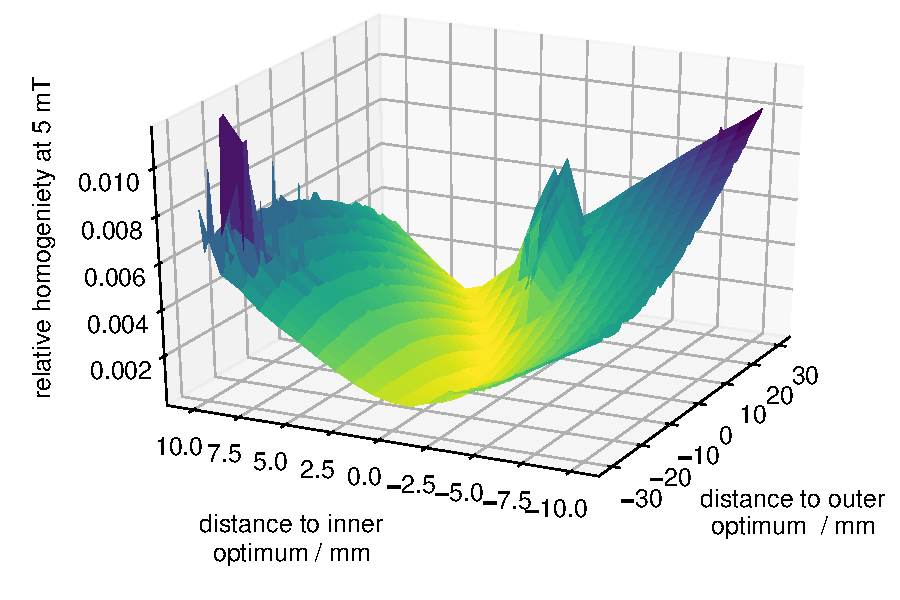
\includegraphics[width = 0.99\textwidth]{/figures/simulations/B0/helmholtzCoil/fieldSpread.pdf}
            \caption[Distance variation homogeniety]{3D plot of the central region of high homogeneity shown in \ref{fig:results:distanceVariation}. Note that the distance variation of the inner coil has a more prominent effect on field homogeneity than the outer one. The minimum value found is a relative spread of $5\cdot 10^{-5}$.}
            \label{fig:results:fieldSpread}
        \end{figure}
        The lowest value found is a relative spread of $4.6 \cdot 10^{-5}$ corresponding to a linewidth of \SI{12.5}{\hertz}. Experimentally, similar values were observed (see chapter \ref{chap:results:lowFieldNMR}). Small variations in the distances lead to strong decrease in homogeneity especially for the inner coil pair - \SI{0.1}{\milli\meter} variations already make up for a decrease of 3 in homogeneity in the inner coil pair while for the outer pair, the same variation makes up for an increase by a factor of 0.2 only. Overall, exact positioning is thus crucial, especially for the inner coil pair. The dual Helmholtz design has thus increased homogeneity to linewidths smaller than those of the solenoid with compensation windings and linear shims. Adding shims to the Helmholtz array is possible and encouraged for future work and will probably further improve homogeneity.
        \subsubsection{Nicotinamide level anti crossings using the spin framework}
        The spin framework developed by Stephan Knecht in this group \cite{knecht_spin_2014} was used to calculate the field dependence of SABRE hyperpolarization for nicotinamide and IR-IMes as a spin system. The results obtained are similar to results previously published concerning pyridine and IR-IMes \cite{hovener_continuous_2014-1}. In figure \ref{figure:results:simulation:nicotinamideSpinSystem} the polarization levels are plotted against field and contact time of the complex (i.e. spin evolution time). These results indicate highest polarizations at \SI{4.9}{\milli\tesla} which is close to the optimum field when using pyridine as the substrate. A contact time of \SI{10}{\milli\second} seems best to generate high polarizations which can be controlled indirectly via the sample temperatures. These results were used to adjust experimental parameters in the best possible way and were confirmed through field variations.
        \begin{figure}
            \centering
            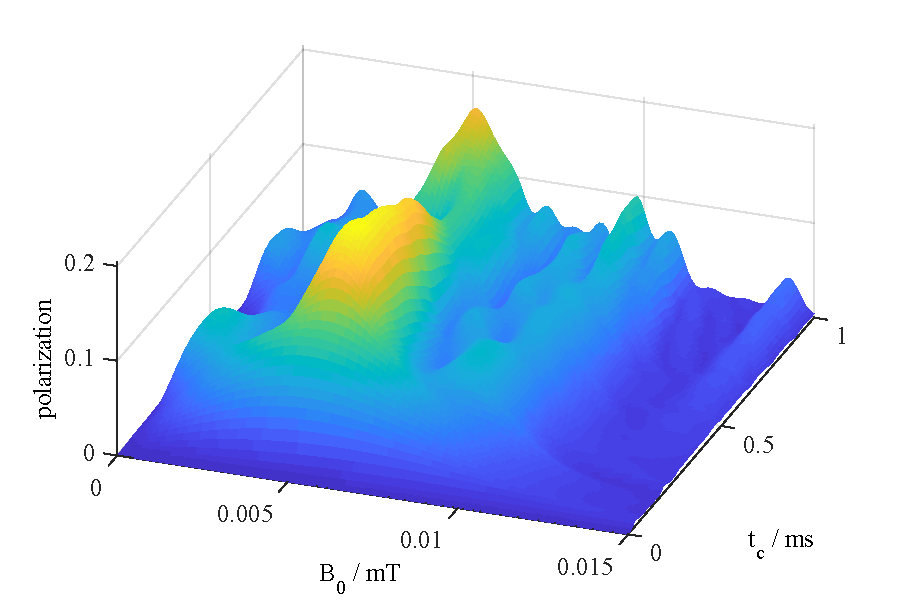
\includegraphics[width=0.99\textwidth]{/figures/simulations/15NSabre/spinFramework/fieldContactTimeDependence.pdf}
            \caption[Spin density matrix calculations]{The }
            \label{figure:results:simulation:nicotinamideSpinSystem}
        \end{figure}
